\documentclass[12pt,letterpaper]{article}
\usepackage[utf8]{inputenc}
\usepackage{amsmath}
\usepackage{amsfonts}
\usepackage{amssymb}
\usepackage{graphicx}
\usepackage{fancybox}
\usepackage{caption}
\usepackage{listings}
\usepackage{hyperref}
\setlength{\captionmargin}{10mm}
\renewcommand\captionfont{\it}
\renewcommand\captionlabelfont{\bf}
\hypersetup{
   pdfauthor = {Kim Siang Khaw},
	colorlinks=true, citecolor=blue, linkcolor=blue, bookmarksnumbered = true,
}
\usepackage[left=2.5cm,right=2.5cm,top=2cm,bottom=2cm]{geometry}
\author{Kim Siang Khaw \\
University of Washington}
\title{\textbf{SLAC 2016 data analysis: Documentation and explanations}}

\begin{document}
\maketitle

\section{Introduction}
Prerequisites for this tutorial are a basic understand of what the Muon g-2 experiment and PbF$_2$ calorimeters are, some knowledge about the electromagnetic (EM) shower
and the ROOT data analysis framework. You can follow the exercise sheet step by step which guides you to the data analysis using the reconstructed electron EM shower clusters.
Some analyses may require the use of reconstructed crystal hit, which is the basic object of forming a cluster. Advanced users may use the FNAL's \textit{art} framework for the data analysis.
%
%trim left bottom right top
\begin{figure}[htbp]
\centering
%\fbox{\includegraphics[trim=0cm 5.5cm 0cm 5.5cm ,width=0.9\textwidth]{pics/EMShower}} guide line for trimming
\includegraphics[trim=3cm 1cm 3cm 0cm, width=0.4\textwidth]{pics/EMShower}
\caption{Illustration of the electromagnetic shower of an electron injected from the left to the right, in a $9\times6$ array PbF$_2$ calorimeter. Cherenkov lights created by the charged shower particles are collected by the Silicon Photomultipliers (SiPMs) glued to the end of the PbF$_2$ crystals.}
\end{figure}

Physics analysis of this test beam has several components that are common to the full Muon g-2 experiment. The physics objects that will be used for most of the analyses are the crystal hits and the clusters.
These objects are reconstructed from the digitized waveform, after going through steps like pulsing fitting, energy calibration, gain correction and hit clustering. During the first week of the test beam, all these reconstruction steps
will be refined based on the data taken and these will be taken care of by those who are familiar with the \textit{art} framework. The main focus of this documentation is on the analysis using high level physics objects like the crystal hit and the cluster.

Several studies that will be covered for the data analysis (non-exhaustive list) are
\begin{itemize}
\item energy resolution of the calorimeter
\item position and angular resolution of the calorimeter
\item degeneracy of the position and angular information of the calorimeter
\item stability of gain monitoring system
\item pile up separation for multi-electron events
\end{itemize}

Further information about how the data will be processed are summarized in Appendix A.

%% For myself
%% Explain the offline data analysis flow here

\section{Data samples}

\subsection{File naming}

The midas run number is preserved for each art/ROOT and ROOT files created from it.  

\begin{table}[htbp]
\centering
\caption{Data samples and descriptions.}
\begin{tabular}{|c|c|} \hline 
filename & type \\ \hline 
run00xxx\_unpacked.root & data ready for art-based analysis \\ \hline 
run00xxx\_analysis.root & data ready for standalone C++ analysis \\ \hline 
\end{tabular} \label{tab:datasamples}
\end{table}

\subsection{Location of the files}

For the following steps, you have to be connected to the local Wifi network \verb+g2SLAC+.
All the art/ROOT and ROOT files are stored in the $2\times3$TB HDD in the \verb+g2analyzer+ machine.
Use the following command to copy over the data files that you want to analyze: 
%
\begin{lstlisting}[frame=single, basicstyle=\ttfamily\footnotesize]
scp -r g2muon@g2analyzer:/data/root_analysis/run00xxx_analysis.root
\end{lstlisting}
%
Or you can use \verb+rsync+ if you have enough space in your hard drive  
%
\begin{lstlisting}[frame=single, basicstyle=\ttfamily\footnotesize]
rsync -avurt g2muon@g2analyzer:/data/root_analysis/ /your/folder/
\end{lstlisting}

\section{Data format and structure for the ROOT tree}
The data samples for this tutorial are stored in ROOT trees. The tree contains a collection of variables (called branches) which are filled once per event (could be 1 or more electrons). The list of variables along with their
data type and further explanations are given in the following. 

\subsection*{For studies using higher level objects}

\begin{itemize}
\item \verb+NCluster+ (int): number of clusters in the event.
\item \verb+Cluster_X+ (double): local x-position of the cluster in the event. 
\item \verb+Cluster_Y+ (double): local y-position of the cluster in the event. 
\item \verb+Cluster_Z+ (double): local z-position of the cluster in the event. 
\item \verb+Cluster_E+ (double): energy (MeV) of the cluster in the event. 
\item \verb+Cluster_T+ (double): time (ns) of the cluster in the event. 

\item \verb+NXtalHit+ (int): number of crystal hits in the event.
\item \verb+XtalHit_X+ (double): local x-position of the crystal hit in the event. 
\item \verb+XtalHit_Y+ (double): local y-position of the crystal hit in the event. 
\item \verb+XtalHit_Z+ (double): local z-position of the crystal hit in the event. 
\item \verb+XtalHit_E+ (double): energy (MeV) of the crystal hit in the event. 
\item \verb+XtalHit_T+ (double): time (ns) of the crystal hit in the event. 
\item \verb+XtalHit_XtalNum+ (int): crystal number in a calorimeter of the crystal hit in the event. 
\end{itemize}

\subsection*{For studies using lower level objects}

\begin{itemize}
\item \verb+Cluster_X+ (double): local x-position of the cluster in the event. 
\item \verb+Cluster_Y+ (double): local y-position of the cluster in the event. 
\item \verb+Cluster_Z+ (double): local z-position of the cluster in the event. 
\item \verb+Cluster_E+ (double): energy (MeV) of the cluster in the event. 

\end{itemize}

\section{Standalone C++ Analysis framework}

The package \verb+SLAC2016Ana.tar.gz+ contains an example \verb+C+++ framework to help you getting started. Unpack the example with \verb+tar xvzf SLAC2016Ana.tar.gz+ to your work folder. You can build your additional analysis code on top of this example or write a new one based on it. The example is already running but it's not doing much yet. You can compile the analysis code by first sourcing your ROOT environment (e.g. \verb+source /usr/local/bin/thisroot.sh+) and then followed by executing the command \verb+make+.

This will read the necessary ingredients for compilation from the \verb+Makefile+ in the same directory. Don't have to worry much about this file at the moment unless you want to add in more classes to the analysis code.
The point is that it creates an executable named \verb+ana+. You can then execute the program by the command \verb+./ana input.script+ where \verb+input.script+ includes a path to the root file that you want to analyze (e.g. \verb+./test.root+). 

A description of the individual components of the example are given in the following list. Indicated are also the places where you should start adding your own code:

\begin{itemize}
\item  \verb+main.cxx+: This is the first starting point. It contains the \verb+main()+ function which is necessary for any \verb+C+++ program. The first step is to create instances of \verb+MyAna()+ class which is implemented in the files \verb+MyAna.h+ and \verb+MyAna.C+ (explained in the next items). The \verb+TChain+ represents the ROOT tree discussed in section 3. The files which should be read from disk are specified in the function \verb+Add(filename)+. The tree is then read and processed by the \verb+MyAna()+ class which takes the \verb+TChain+ as argument. The real work is then done in the \verb+Loop()+ function of the \verb+MyAna()+ class which is discussed in the next two items. 

\item \verb+MyAna.h+: Definition of the class \verb+MyAna+, which inherits from the \verb+TTree::MakeClass+. It declares variables and ROOT objects that will be used or stored in your analysis. Several basic functions that are common among event-based particle physics analysis like \verb+initialize()+, \verb+clear()+, \verb+execute()+ and\verb+finalize()+ are declared here.
%% to myself
%% need to change the names like Loop, execute, etc because it is a bit confusing
\item \verb+MyAna.C+: The main function which is called automatically which processing the ROOT trees are \verb+Loop()+. The \verb+Loop()+ function is called only once per run. In the \verb+Loop()+ function, \verb+initialize()+ is called at the beginning of the analysis run, \verb+clear()+ and \verb+execute()+ is called every event, and \verb+finalize()+ at the end of the analysis run.

\item \verb+t1.h+: Header file for the class \verb+t1+ created using \verb+TTree::MakeClass+.  

\item \verb+t1.C+: Source file for the class \verb+t1+ created using \verb+TTree::MakeClass+. The class \verb+Loop()+ is used by \verb+MyAna+ to loop through each \verb+TBranch+.

\item \verb+PlotAll.C+: A ROOT macro which can be used for automatic plotting of a set of histograms which are stored in a ROOT file. Please read the header of the file on how to use it. 
\end{itemize}


\section{ROOT-based offline event display}

A ROOT-based offline event display is also developed to increase the user friendliness of the data analysis. As shown in Figure~\ref{fig:GUI}, this GUI interface allows the user to inspect the fit results of the template fit algorithm by overlaying it with the island samples.
More functionality will be added in the coming days.

\begin{figure}[htbp]
\centering
%\fbox{\includegraphics[trim=0cm 5.5cm 0cm 5.5cm ,width=0.9\textwidth]{pics/EMShower}} guide line for trimming
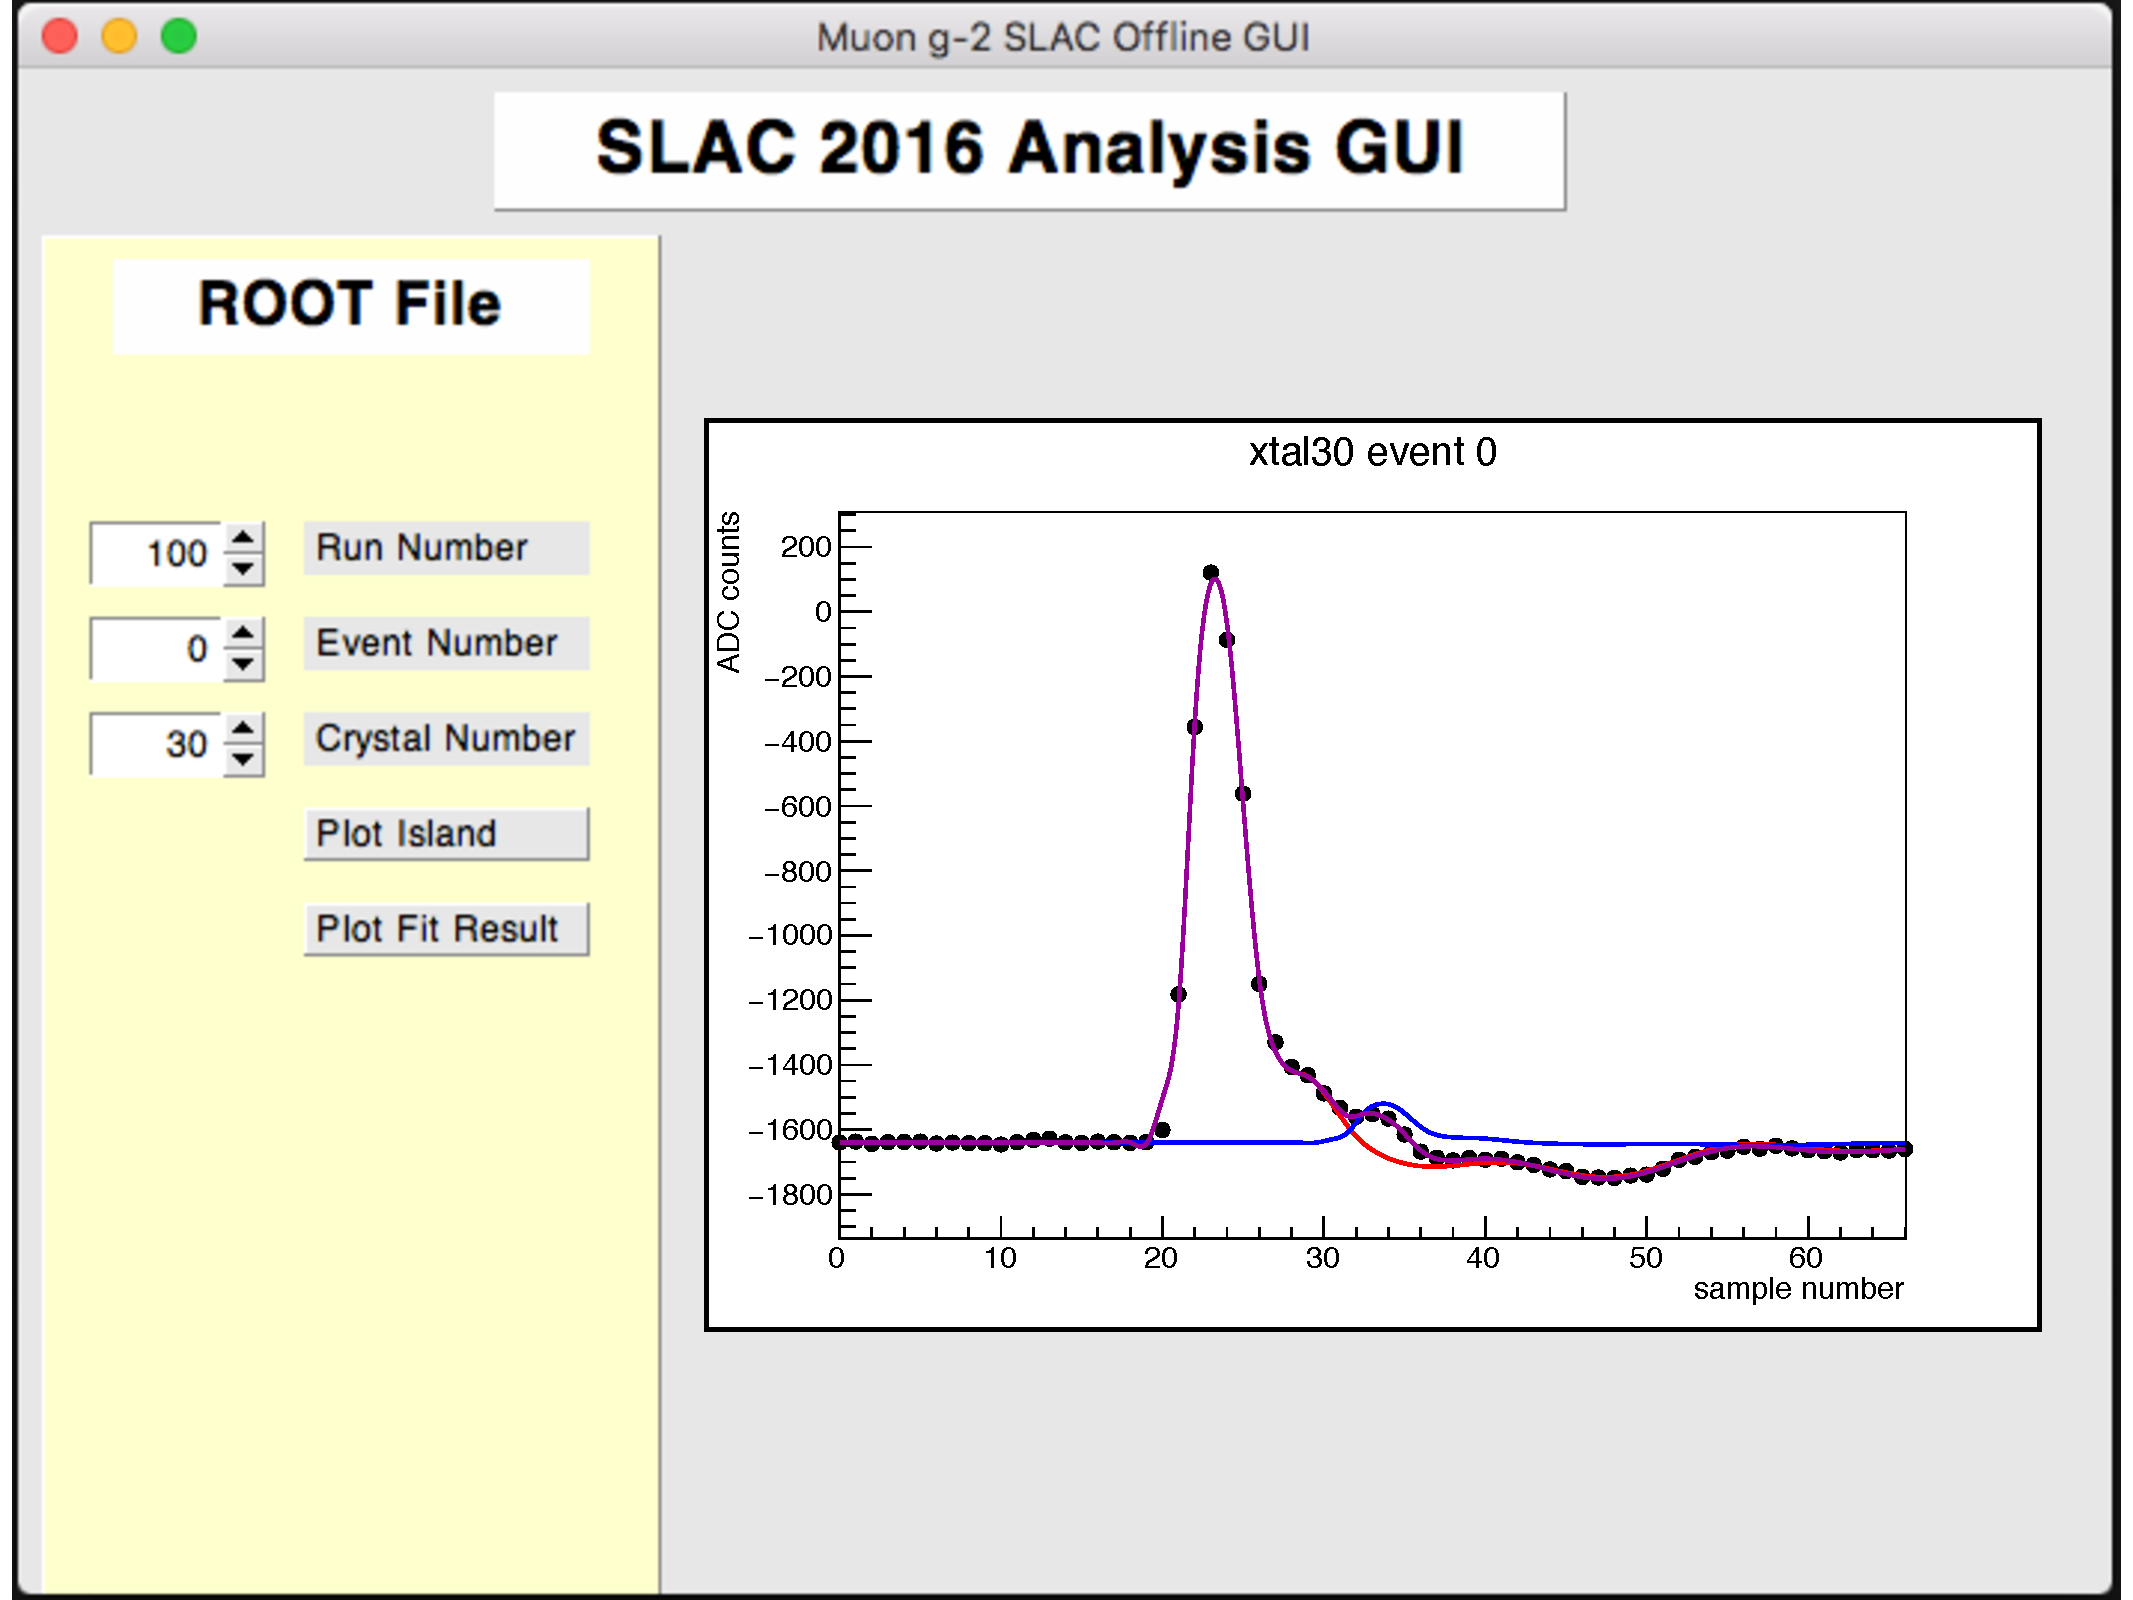
\includegraphics[width=0.75\textwidth]{pics/SLAC2016_Analysis_GUI}
\caption{SLAC Offline analysis GUI. This is a very preminary prototype.}\label{fig:GUI}
\end{figure}


\newpage
\appendix

\section{Data analysis framework}

\begin{figure}[htbp]
\centering
%\fbox{\includegraphics[trim=0cm 5.5cm 0cm 5.5cm ,width=0.9\textwidth]{pics/EMShower}} guide line for trimming
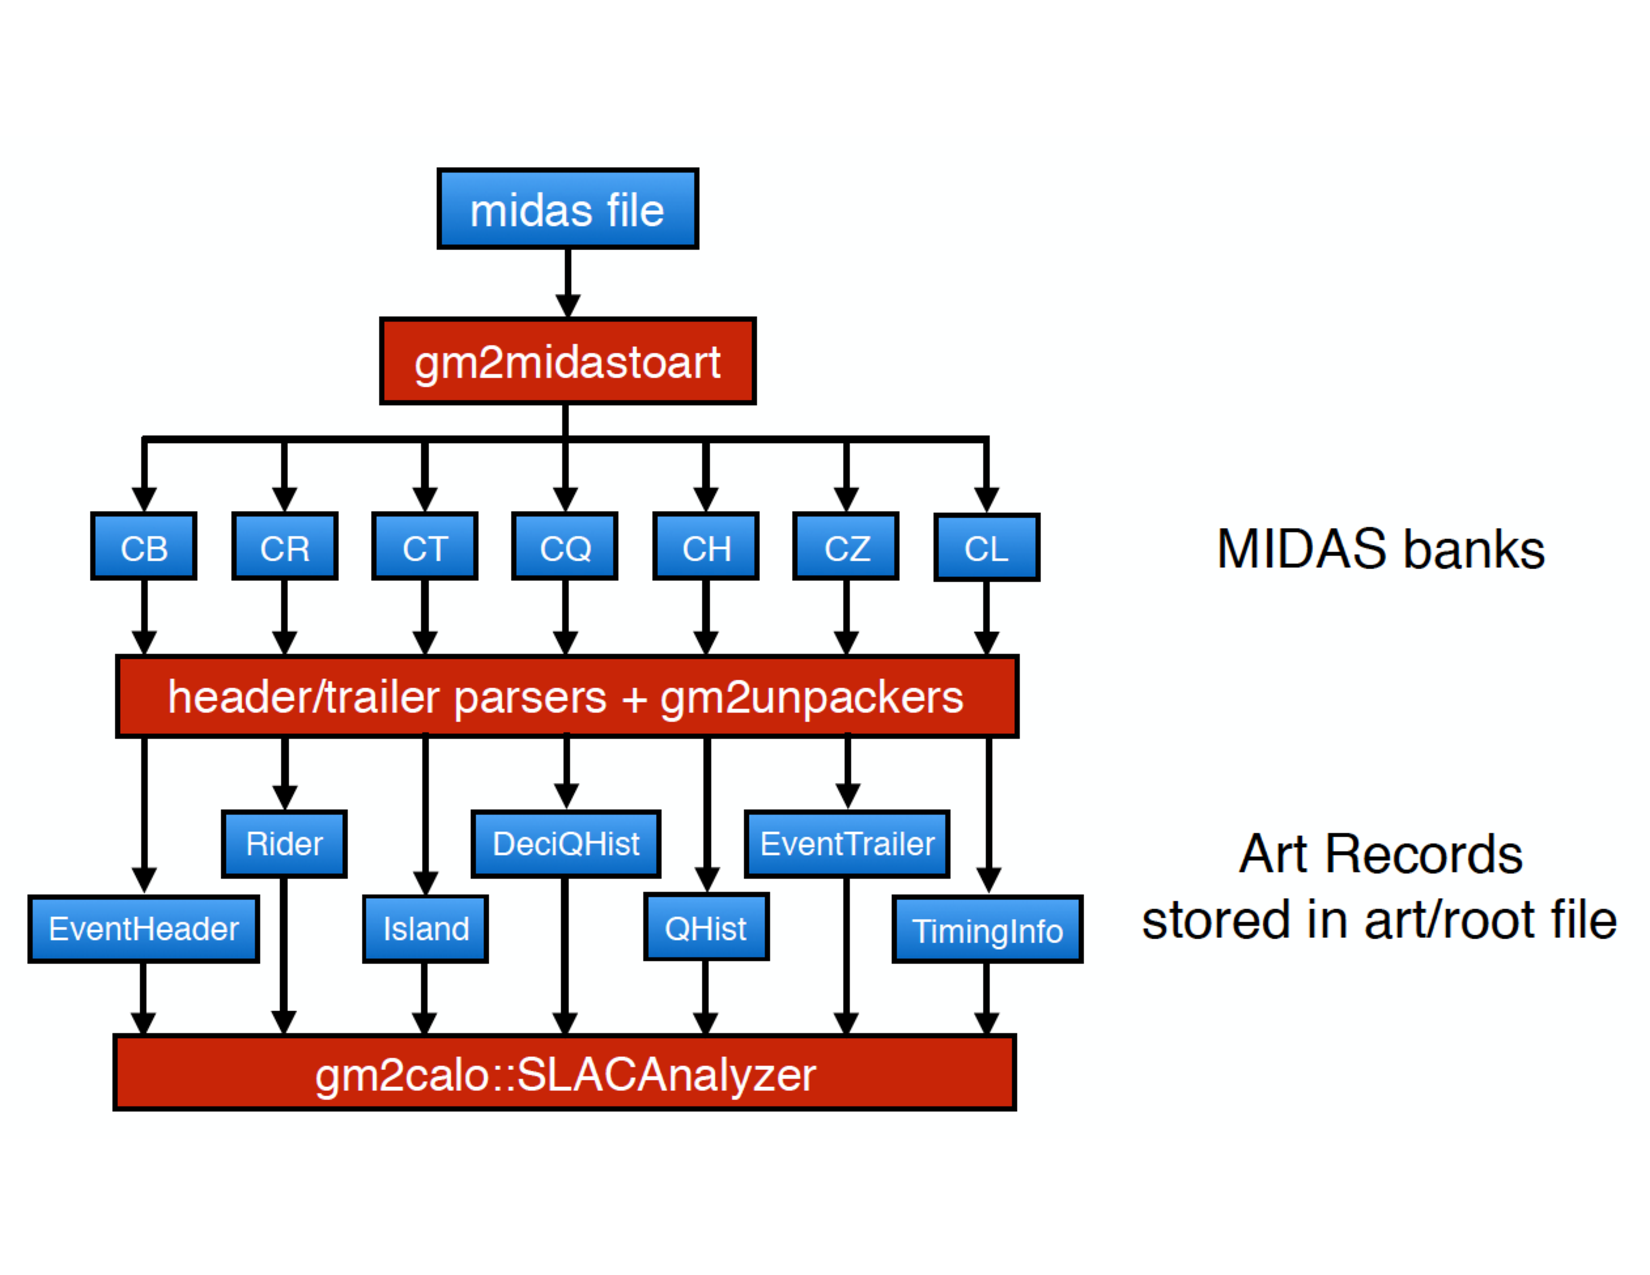
\includegraphics[width=0.8\textwidth]{pics/offline_slac_framework}
\caption{Offline framework for SLAC experimental data.}
\end{figure}

The data analysis of this test beam has several components. First we need to convert the raw data stored in a MIDAS file (\verb+.mid+ or \verb+.mid.gz+) to \textit{art} data products stored in a ROOT file.
This is handled using \textit{art} framework's modules and is doing nothing more than storing \verb+16-bit+ or \verb+32-bit+ word into \verb+vectors+. Next we unpack these \verb+vectors+
and give them contexts based on the header information stored within the \verb+vectors+. As this step, all the information are stored as data products you are probably familiar with: \verb+RiderArtRecord+,
 \verb+IslandArtRecord+, etc.

\section{Header information}
This section provides the information regarding user interface to the event, AMC13 and rider header information. All the information are stored in the art/ROOT files and standalone ROOT files with the TBranch structures in the following sections.

\subsection{Terminology}
Several technical terms defined in this document. A run consists of multiple events. There is a maximum of 12 AMC slots per calorimeter. Each AMC slot has a Rider digitizer, and each Rider has 5 input channels.

%\newpage
\subsection{RunHeader Class Reference}
Run header appears once for each run.

\subsubsection*{TLeaf members}

Below are the member variables that appear under TBranch RunHeader.

\begin{itemize}
\item ULong\_t \textbf{RunNum}
\item ULong\_t \textbf{NumOfEvent}
\item ULong\_t \textbf{NumOfAMC13Trig}
\item ULong\_t \textbf{NumOfRiderTrig}
\end{itemize}

%\newpage
\subsection{EventHeader Class Reference}
Event header appears once for each event.

\subsubsection*{TLeaf members}

Below are the member variables that appear under TBranch EventHeader.

\begin{itemize}
\item ULong\_t \textbf{EventNum}
\item ULong\_t \textbf{AMC13TrigNum}
\item UChar\_t \textbf{EventType}
\item UChar\_t \textbf{NumOfAMC}
\item UChar\_t \textbf{NumOfRiderChannel}
\item struct \textbf{AMCHeader} 
    \begin{itemize}
    \item UChar\_t \textbf{AMCSlotNum}  
    \item ULong\_t  \textbf{RiderSerialNum}  
    \item ULong\_t \textbf{AMCCounter}
    \item ULong\_t \textbf{RiderTrigNum}
    \end{itemize} 
\end{itemize}

%\newpage
\subsection{RiderChannelHeader Class Reference} 
Rider channel header appears once for each rider channel.

\subsubsection*{TLeaf members}

Below are the member variables that appear under TBranch RiderChannelHeader.

\begin{itemize}
\item struct \textbf{RiderChannelHeader}
      \begin{itemize}
    \item UChar\_t \textbf{AMCSlotNum}
    \item UChar\_t \textbf{RiderChannelNum}
    \item UChar\_t \textbf{FillType}
     \item ULong\_t \textbf{WaveformIndex}
    \item ULong\_t \textbf{WaveformCount}
    \item ULong\_t \textbf{TriggerNum}
    \item UInt\_t \textbf{WaveformLength}
    \end{itemize}
\end{itemize}


\section{Header and trailer formats}

This section compiles all the available header data formats. Please refer to \url{http://gm2-docdb.fnal.gov:8080/cgi-bin/ShowDocument?docid=3409} for more details.

\begin{figure}[htbp]
\centering
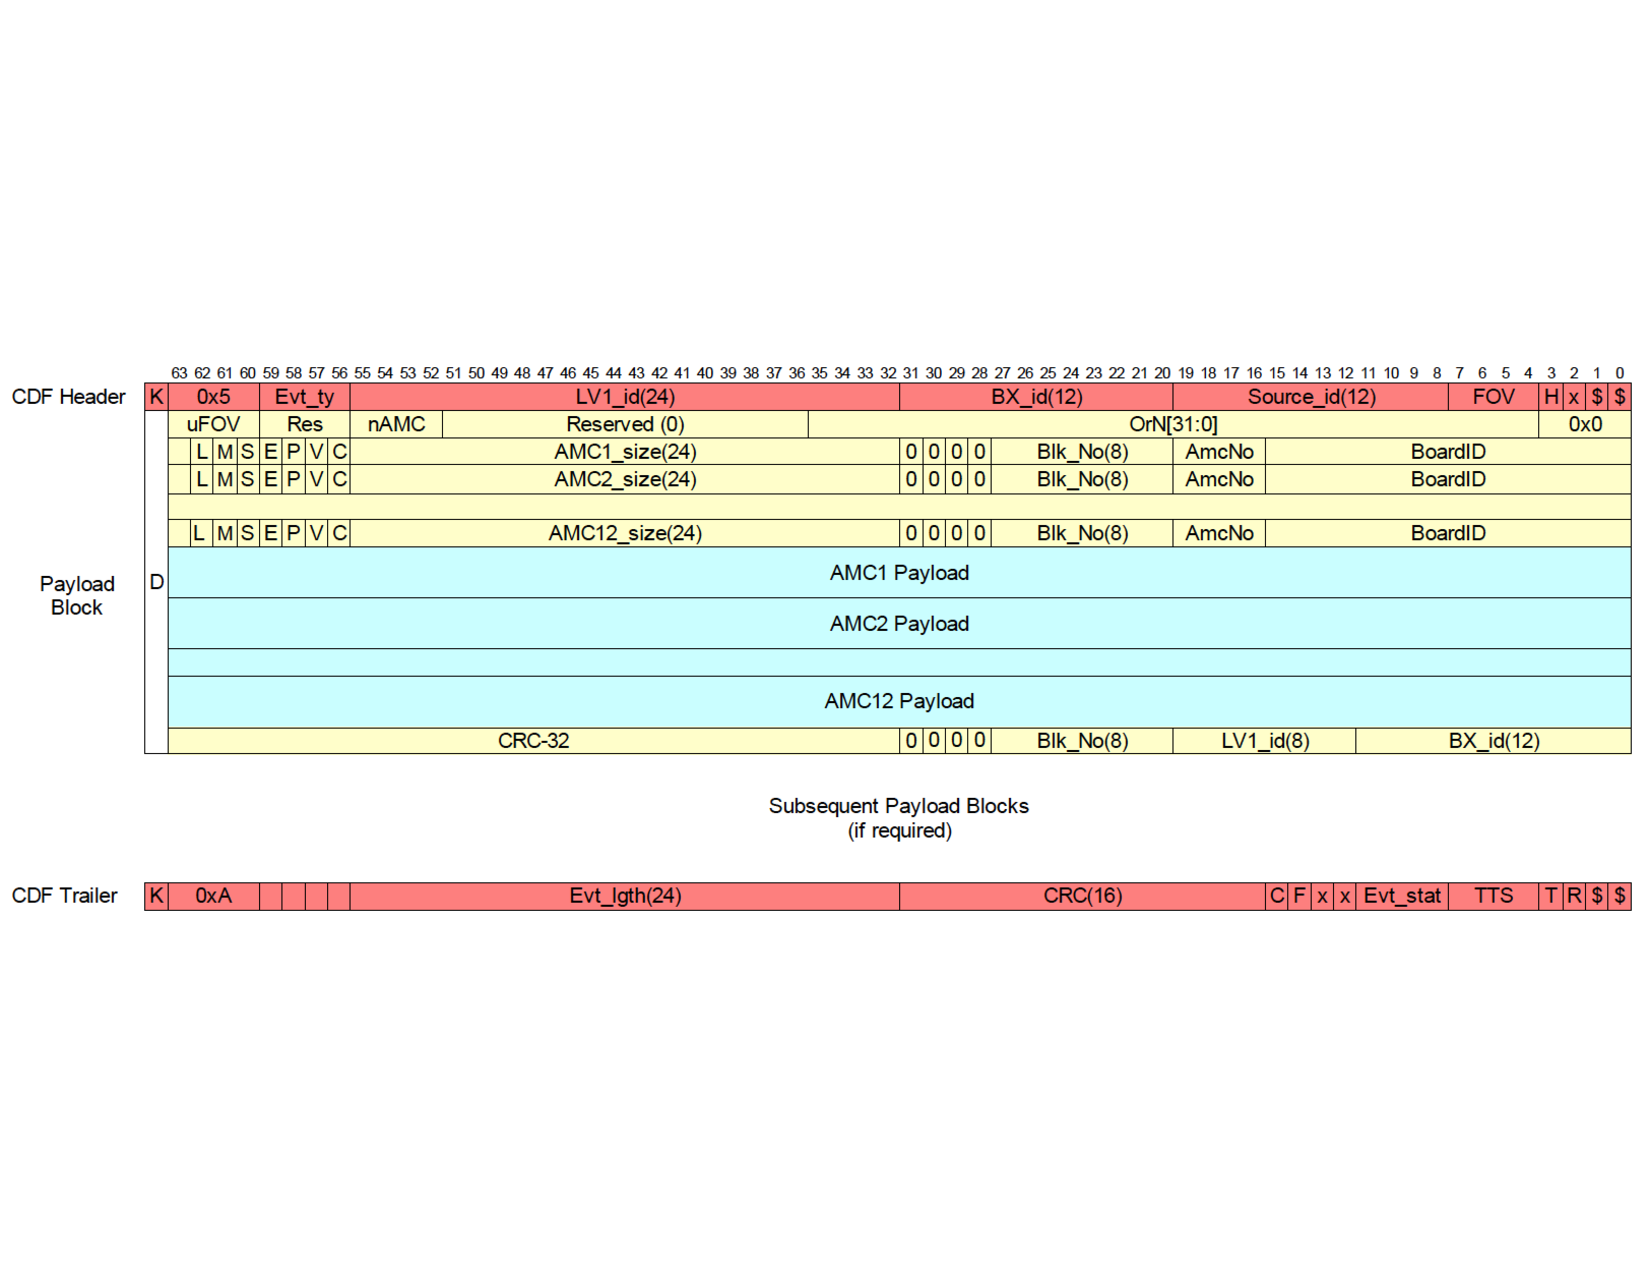
\includegraphics[trim=0cm 6cm 0cm 6cm ,width=0.95\textwidth]{pics/AMC13Header}
\caption{AMC13 to DAQ data format.}
\end{figure}

\begin{figure}[htbp]
\centering
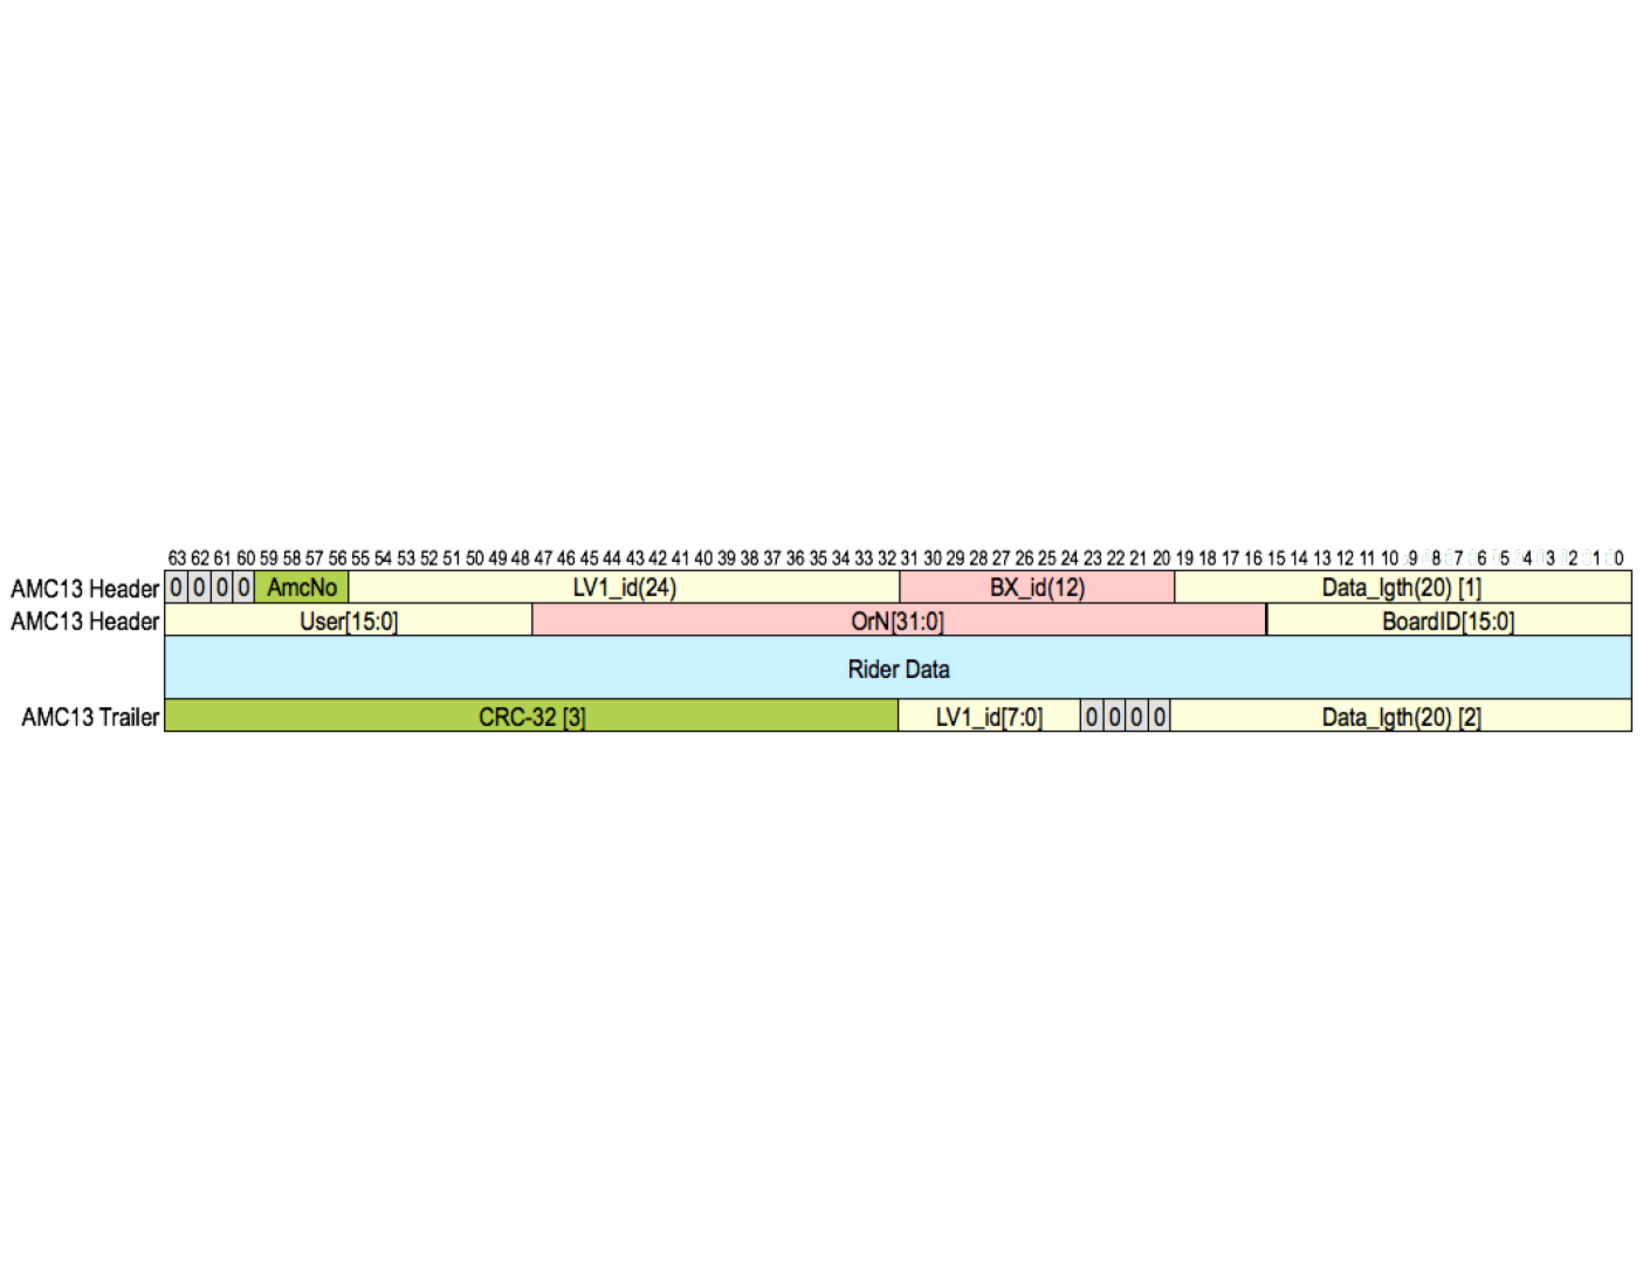
\includegraphics[trim=0cm 9.5cm 0cm 9.5cm ,width=0.95\textwidth]{pics/RiderToAMC13Header}
\caption{Rider to AMC13 data format.}
\end{figure}

%trim left bottom right top
\begin{figure}[htbp]
\centering
%\fbox{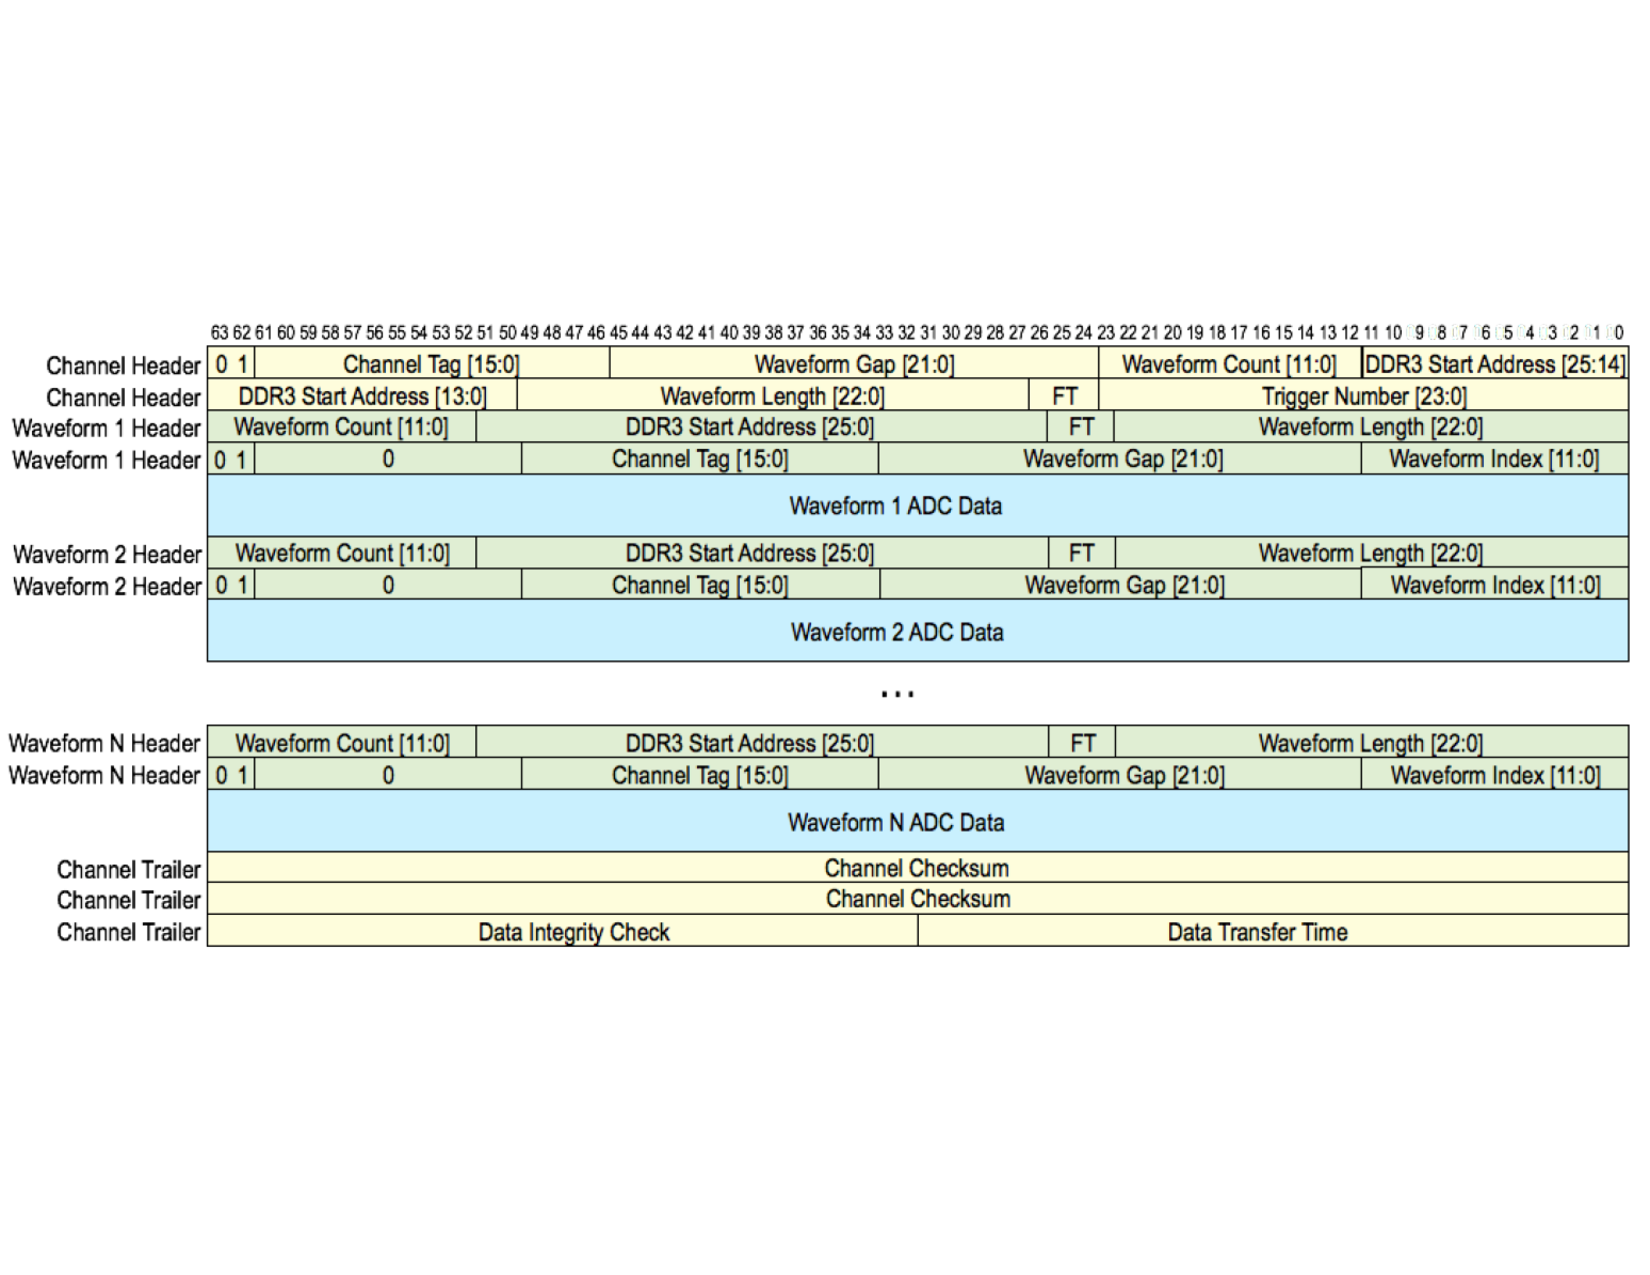
\includegraphics[trim=0cm 5.5cm 0cm 5.5cm ,width=0.9\textwidth]{pics/RiderChannelHeader}} guide line for trimming
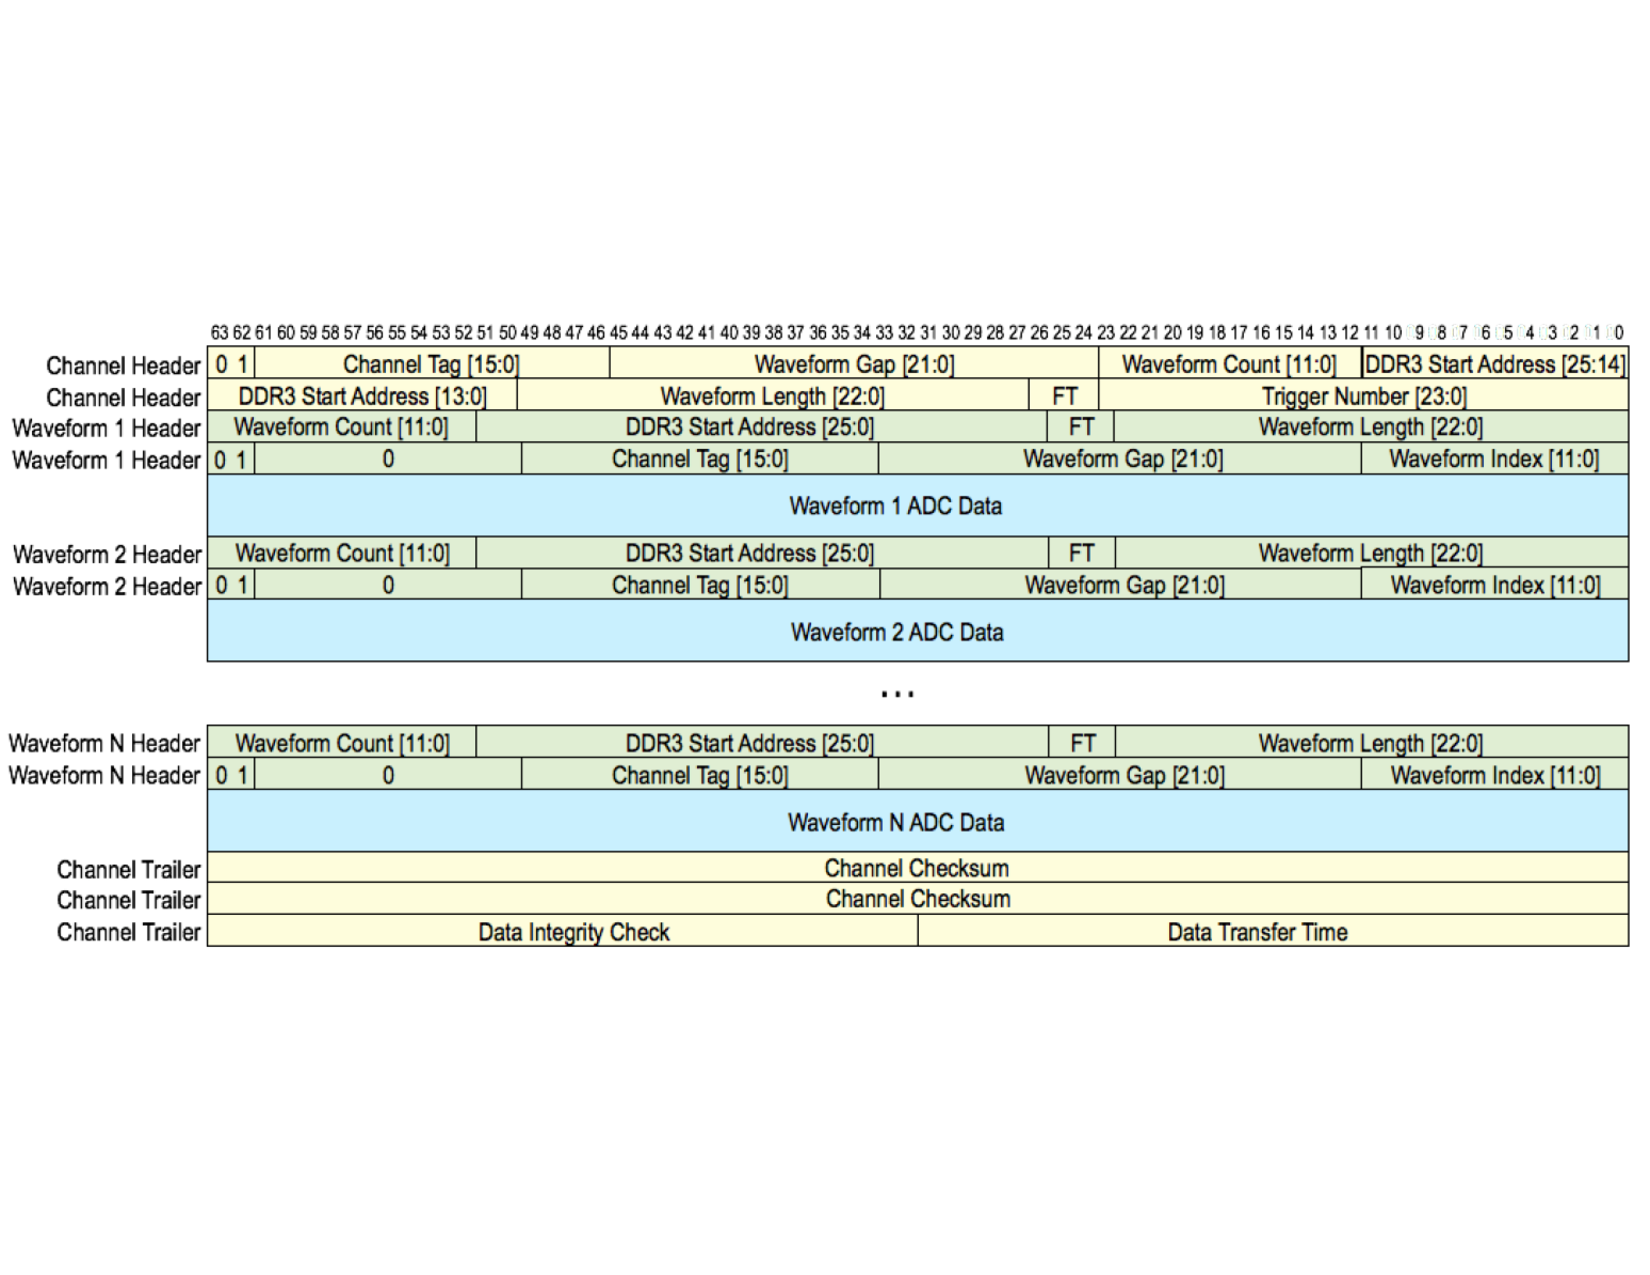
\includegraphics[trim=0cm 5.5cm 0cm 5.5cm ,width=0.95\textwidth]{pics/RiderChannelHeader}
\caption{Rider Channel data format.}
\end{figure}

\begin{figure}[htbp]
\centering
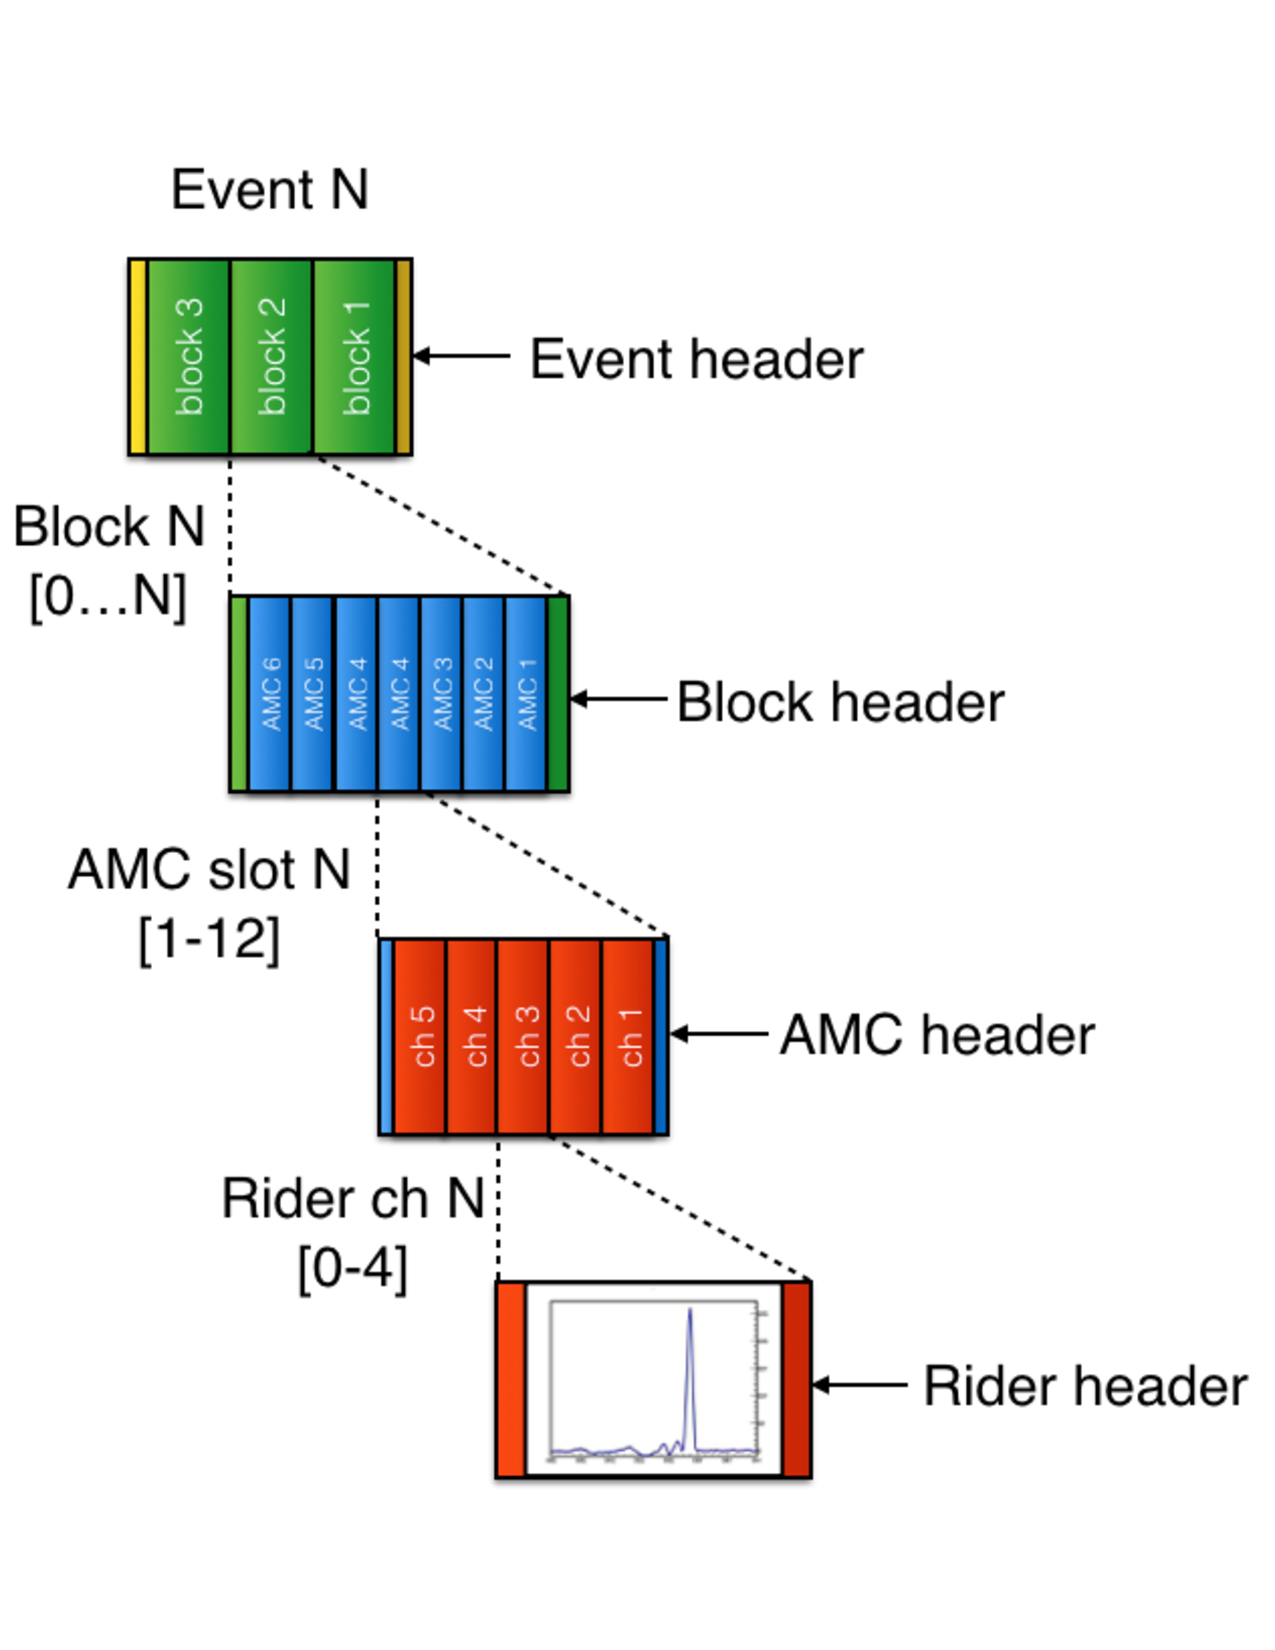
\includegraphics[width=0.9\textwidth]{pics/AllHeaders}
\caption{Per event data format}
\end{figure}


\end{document}

